\graphicspath{{images/}}

\section{\thesection~Results}
\label{sec:results}


\subsection{\thesubsection~Guessing}

\(N_{0}\) estimated from average final cell amounts. See formula in code
for two \(N_{0}\) estimation.

\graphicspath{{images/guessing/}}
\begin{Figure}
  \centering
  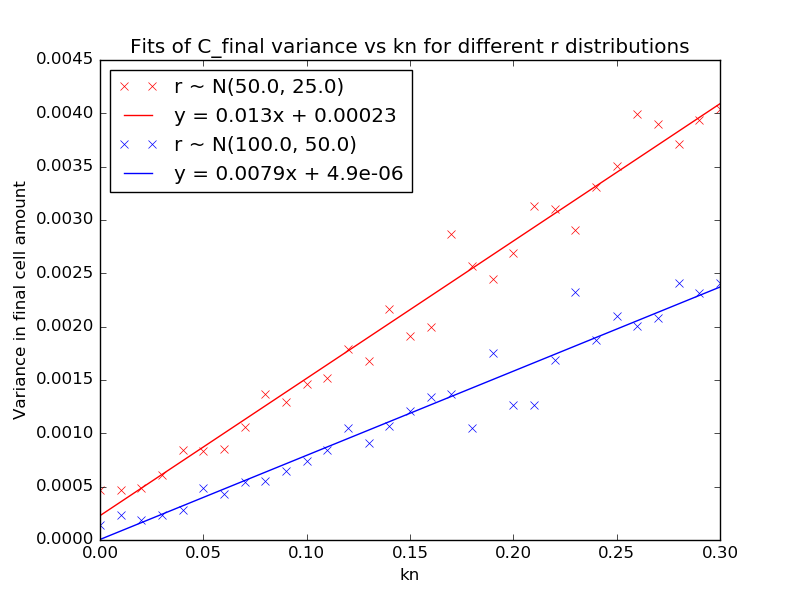
\includegraphics[width=\linewidth]{final/kn_guessing}
  \captionof{figure}{\textbf{Guessing \(k_{n}\) from the variance in
      final cell amounts.} The competition model is simulated for a
    16x24 format plate using two random sets of culture-level \(b\)
    parameters drawn from different normal distributions. Each set of
    \(b\) parameters is simulated with a range of \(k_n\) parameter
    values. The variance in final cell density for all cultures is
    plotted against \(k_n\) for each simulation. Lines are shown for
    least squares fits to points from each set of \(b\) parameters.}
  \label{fig:kn_guessing}
\end{Figure}


\end{multicols}
\graphicspath{{images/guessing/}}
\begin{Figure}
  \centering
  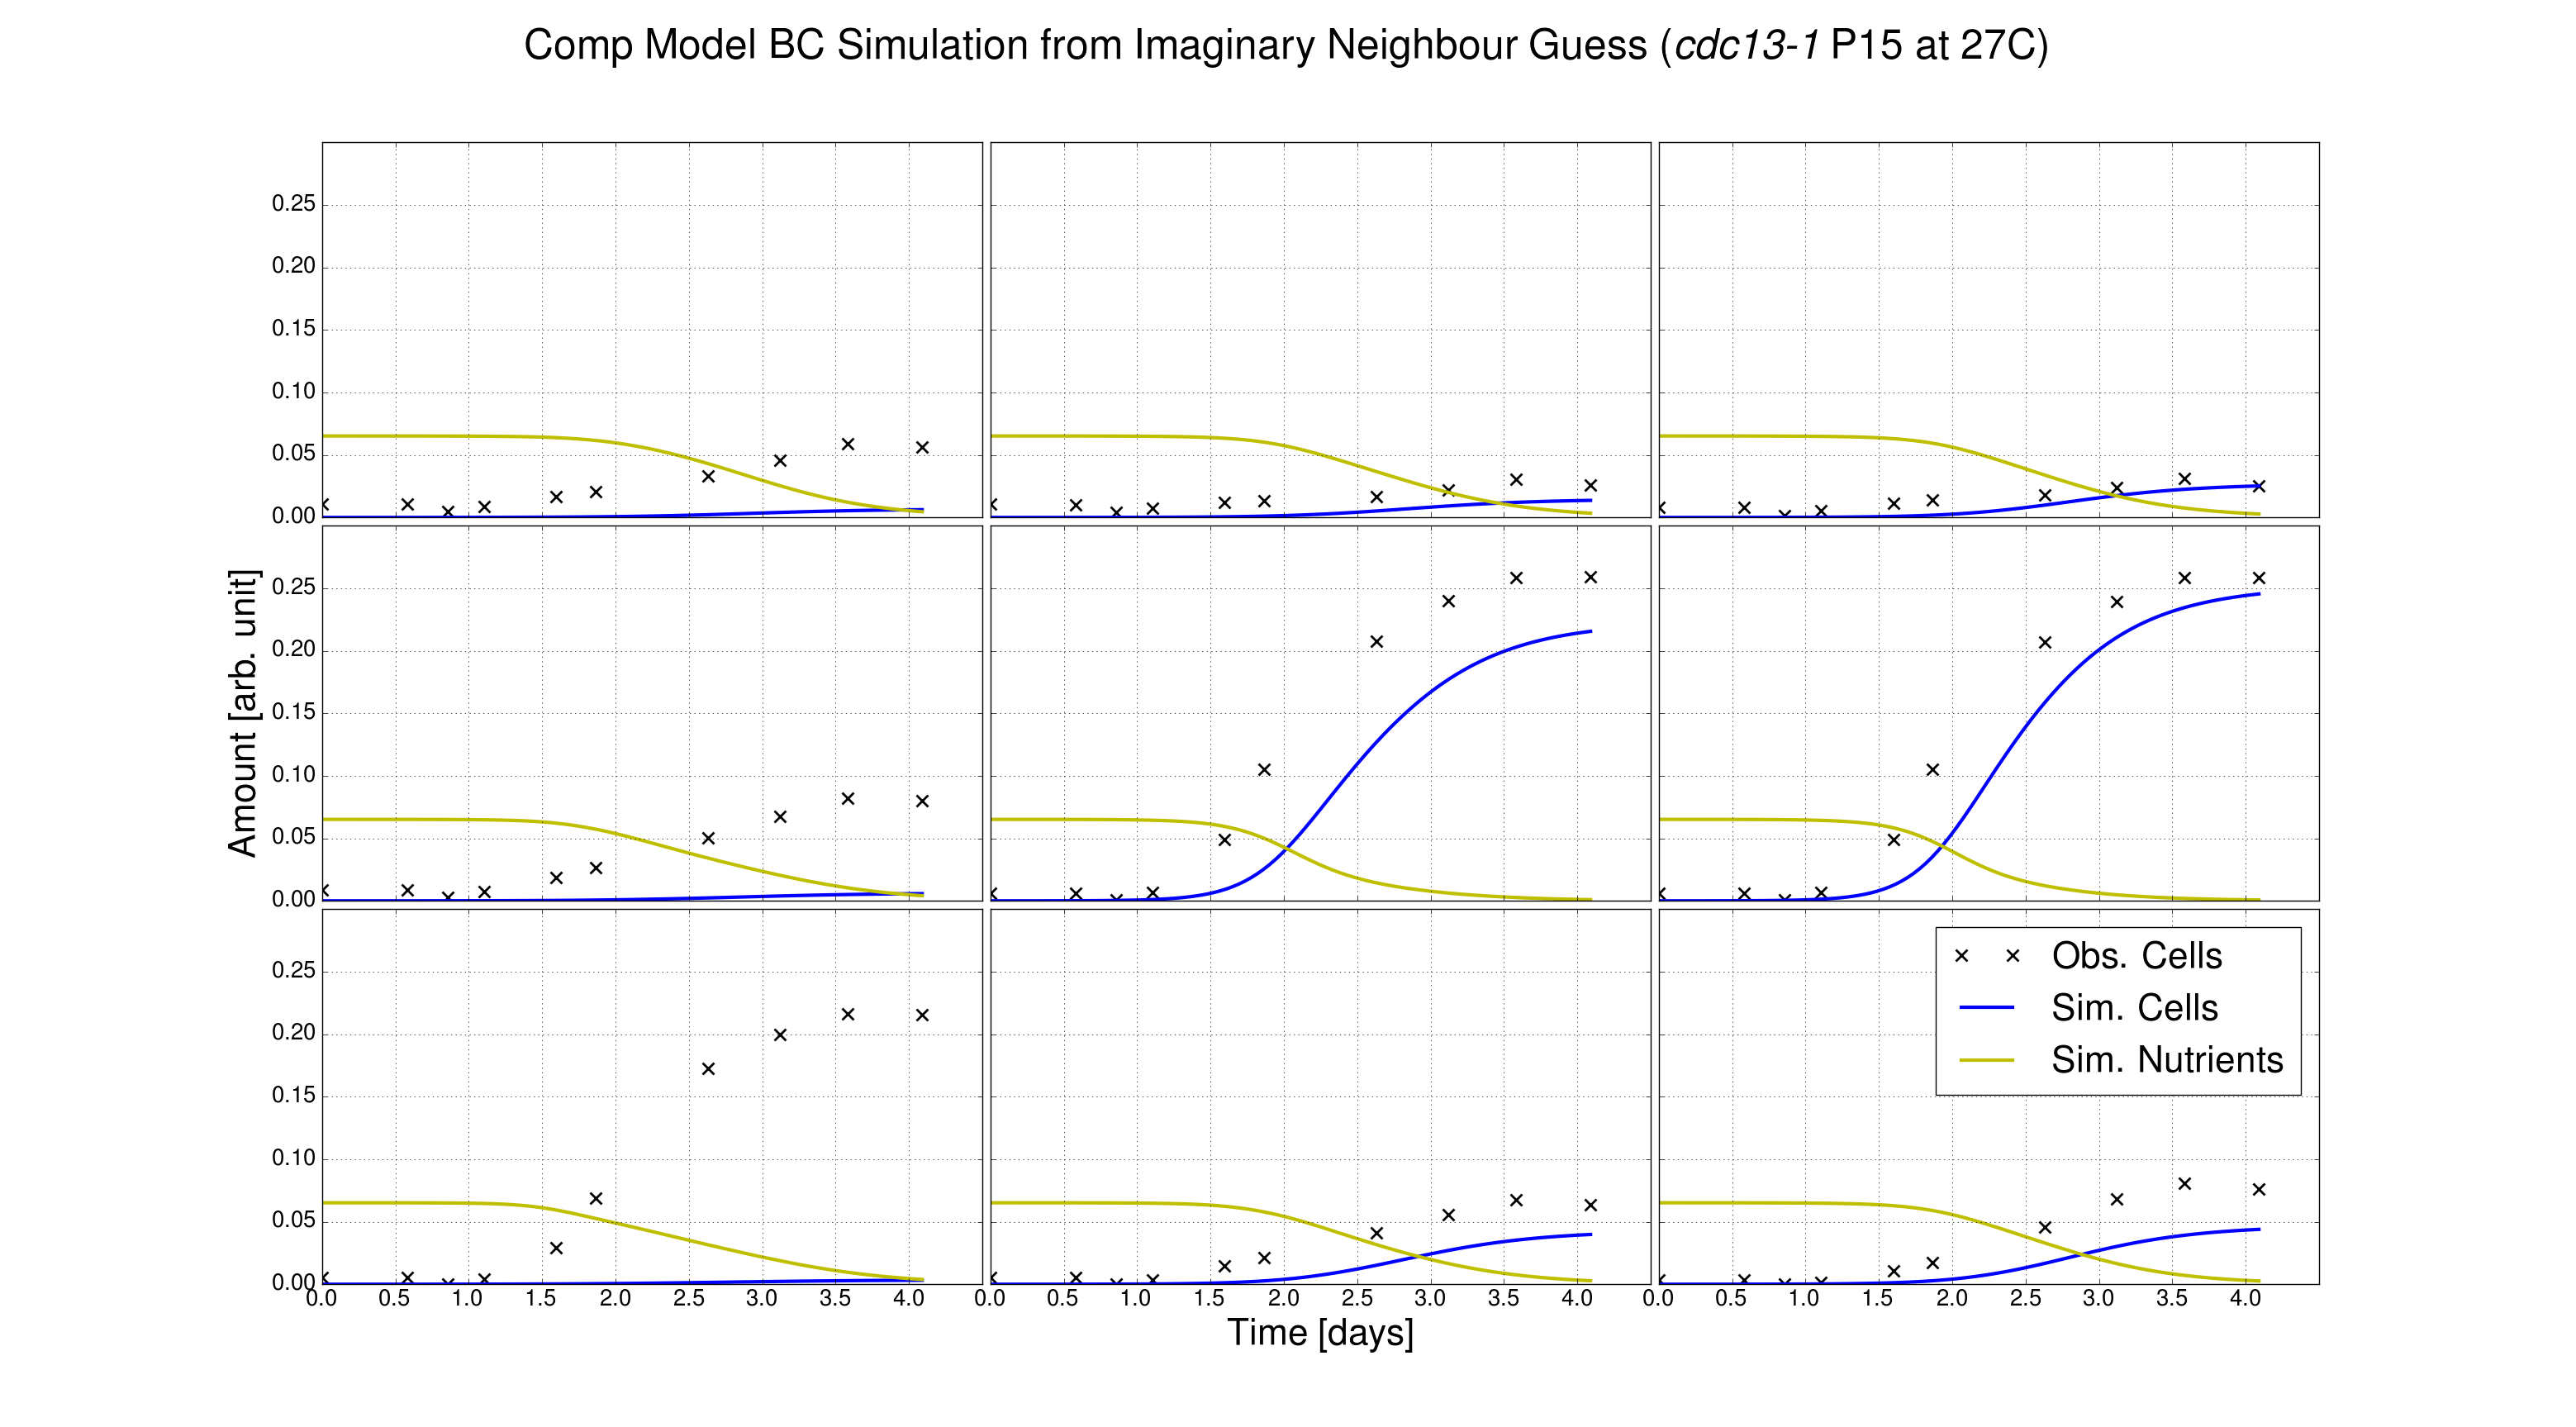
\includegraphics[width=\linewidth]{final/P15_R5_C18_guess_sim}
  \captionof{figure}{\textbf{Competition model simulation using
      parameters from imaginary neighbour guessing.} Shows a 3x3 zone
    with top-left coordinate (5, 18) from P15 with background
    \textit{cdc13-1} at 27\(^{\circ}C\).}
  \label{fig:imag_neigh_guess_sim}
\end{Figure}
\begin{multicols}{2}


  (NOT TO GO HERE This method of guessing requires a b-guess to be
  supplied to fix the faster growi ng neighbour. (I iterated through
  cell ratios. I iterated through a range of b guesses supplied at the
  plate level; running a different script with a \(C_{0}\) guess,
  \(b_{guess}\). It would probably have been better iterate through a
  list of b-guess values for each culture and choosing the estimated b
  value from the best fit of each culture. Guessing time is currently
  about four minutes which is fast compared to fitting which takes
  approximately three hours. However, this is unlikely to stop us from
  encountering local minima when we fit the Competition Model.)

Scripts were run with combinations of the following values.
cellratios = np.logspace(-3, -5, num=5)
fittype = ["imagneigh", "logeq"]
zerokn = [True, False]

Each script looped through the following array of b values which were
supplied to the initial guesser and used at the plate level.

for b-guess in [35, 40, 45, 50, 55, 60, 65, 70, 75, 80, 95, 100, 150]:

Each b-guess value is used to guess a complete set of b parameters for
every culture in the plate. Each of these parameter sets is then used
as an initial guess to Competition Model fitting. For the 13 b-guesses
we must run 13 Competition Model fits. It would be better and more
efficient to loop through the b-guesses at the culture level. Each
culture still undergoes imaginary neighbour guessing with each of the
13 b-guess values, but now, for each culture, we choose just the b
estimate from the best of the 13 fits. This will produce one set of b
guesses which should be superior to any of the guesses attained when
iterating through b-guess at the plate level. Then we only need to fit
the Competition Model to 1 guess rather than 13. This will reduce the
number of scripts that need to be run in parallel, or the use of a
finer grid over \(C_{0}\), and should make convergence
faster. However, if using a gradient method we are still likely to
encounter local minima from these guesses. Instead, this improvement
could be considered when developing a genetic algorithm (if initial
guesses are required) or if fitting using a brute force method with a
fine grid of fixed plate level parameters. We will see later that with
true plate level parameters fixed we can recover good estimates for b
using a gradient method. It may be possible to evolve candidates of
plate level parameters, fix these, and minimise using the current
gradient method.


\subsection{\thesubsection~Competition Model Fitting to P15}

% Make landscape and take a whole page.
\end{multicols}
\begin{landscape}
\graphicspath{{images/comp_fit/}}
\begin{Figure}
  \centering
  \includegraphics[width=\linewidth]{full_plate/final/P15_12x20}
  \captionof{figure}{\textbf{Fit of the competition model to a QFA
      plate.} Data is for a 16x24 format plate (P15) with a background
    mutation \textit{cdc13-1} incubated at 27\(^{\circ}C\). The plate
    contains 6 repeats of 50 genetic strains randomly arranged across
    the internal cultures. Repeats of a single strain are used for all
    edge cultures (removed in the plot). Model output for state
    variable, cell population size (blue curve), is fit to observed
    data (black crosses). Model predictions for unobserved variable
    (nutrient amount) are also plotted (yellow).}
  \label{fig:comp_fit_plate}
\end{Figure}
\end{landscape}
\begin{multicols}{2}

\end{multicols}
\graphicspath{{images/comp_fit/}}
\begin{Figure}
  \centering
  \includegraphics[width=\linewidth]{final/P15_r5_c18_3x3}
  \captionof{figure}{\textbf{A 3x3 zone from Figure~\ref{fig:comp_fit_plate}
      with top-left coordinate (5, 18)}.}
  \label{fig:comp_fit_zone}
\end{Figure}
\begin{multicols}{2}

  Some text Some text Some text Some text Some text Some text Some
  text Some text Some text Some text Some text Some text Some text
  Some text Some text Some text Some text Some text Some text Some
  text Some text Some text Some text Some text Some text Some text
  Some text Some text Some text Some text Some text Some text Some
  text Some text Some text Some text Some text Some text Some text
  Some text Some text Some text Some text Some text Some text Some
  text Some text Some text Some text Some text Some text Some text
  Some text Some text Some text Some text Some text Some text Some
  text Some text Some text Some text Some text Some text Some text
  Some text Some text Some text Some text Some text Some text Some
  text Some text Some text Some text Some text Some text Some text
  Some text Some text Some text Some text Some text Some text Some
  text Some text Some text Some text Some text Some text Some text
  Some text Some text Some text Some text Some text Some text Some
  text Some text Some text Some text Some text Some text Some text
  Some text Some text Some text Some text.


\subsection{\thesubsection~Evaluating the treatment of boundaries}

% should remove title from plot?
\end{multicols}
\graphicspath{{images/corners/}}
\begin{Figure}
  \centering
  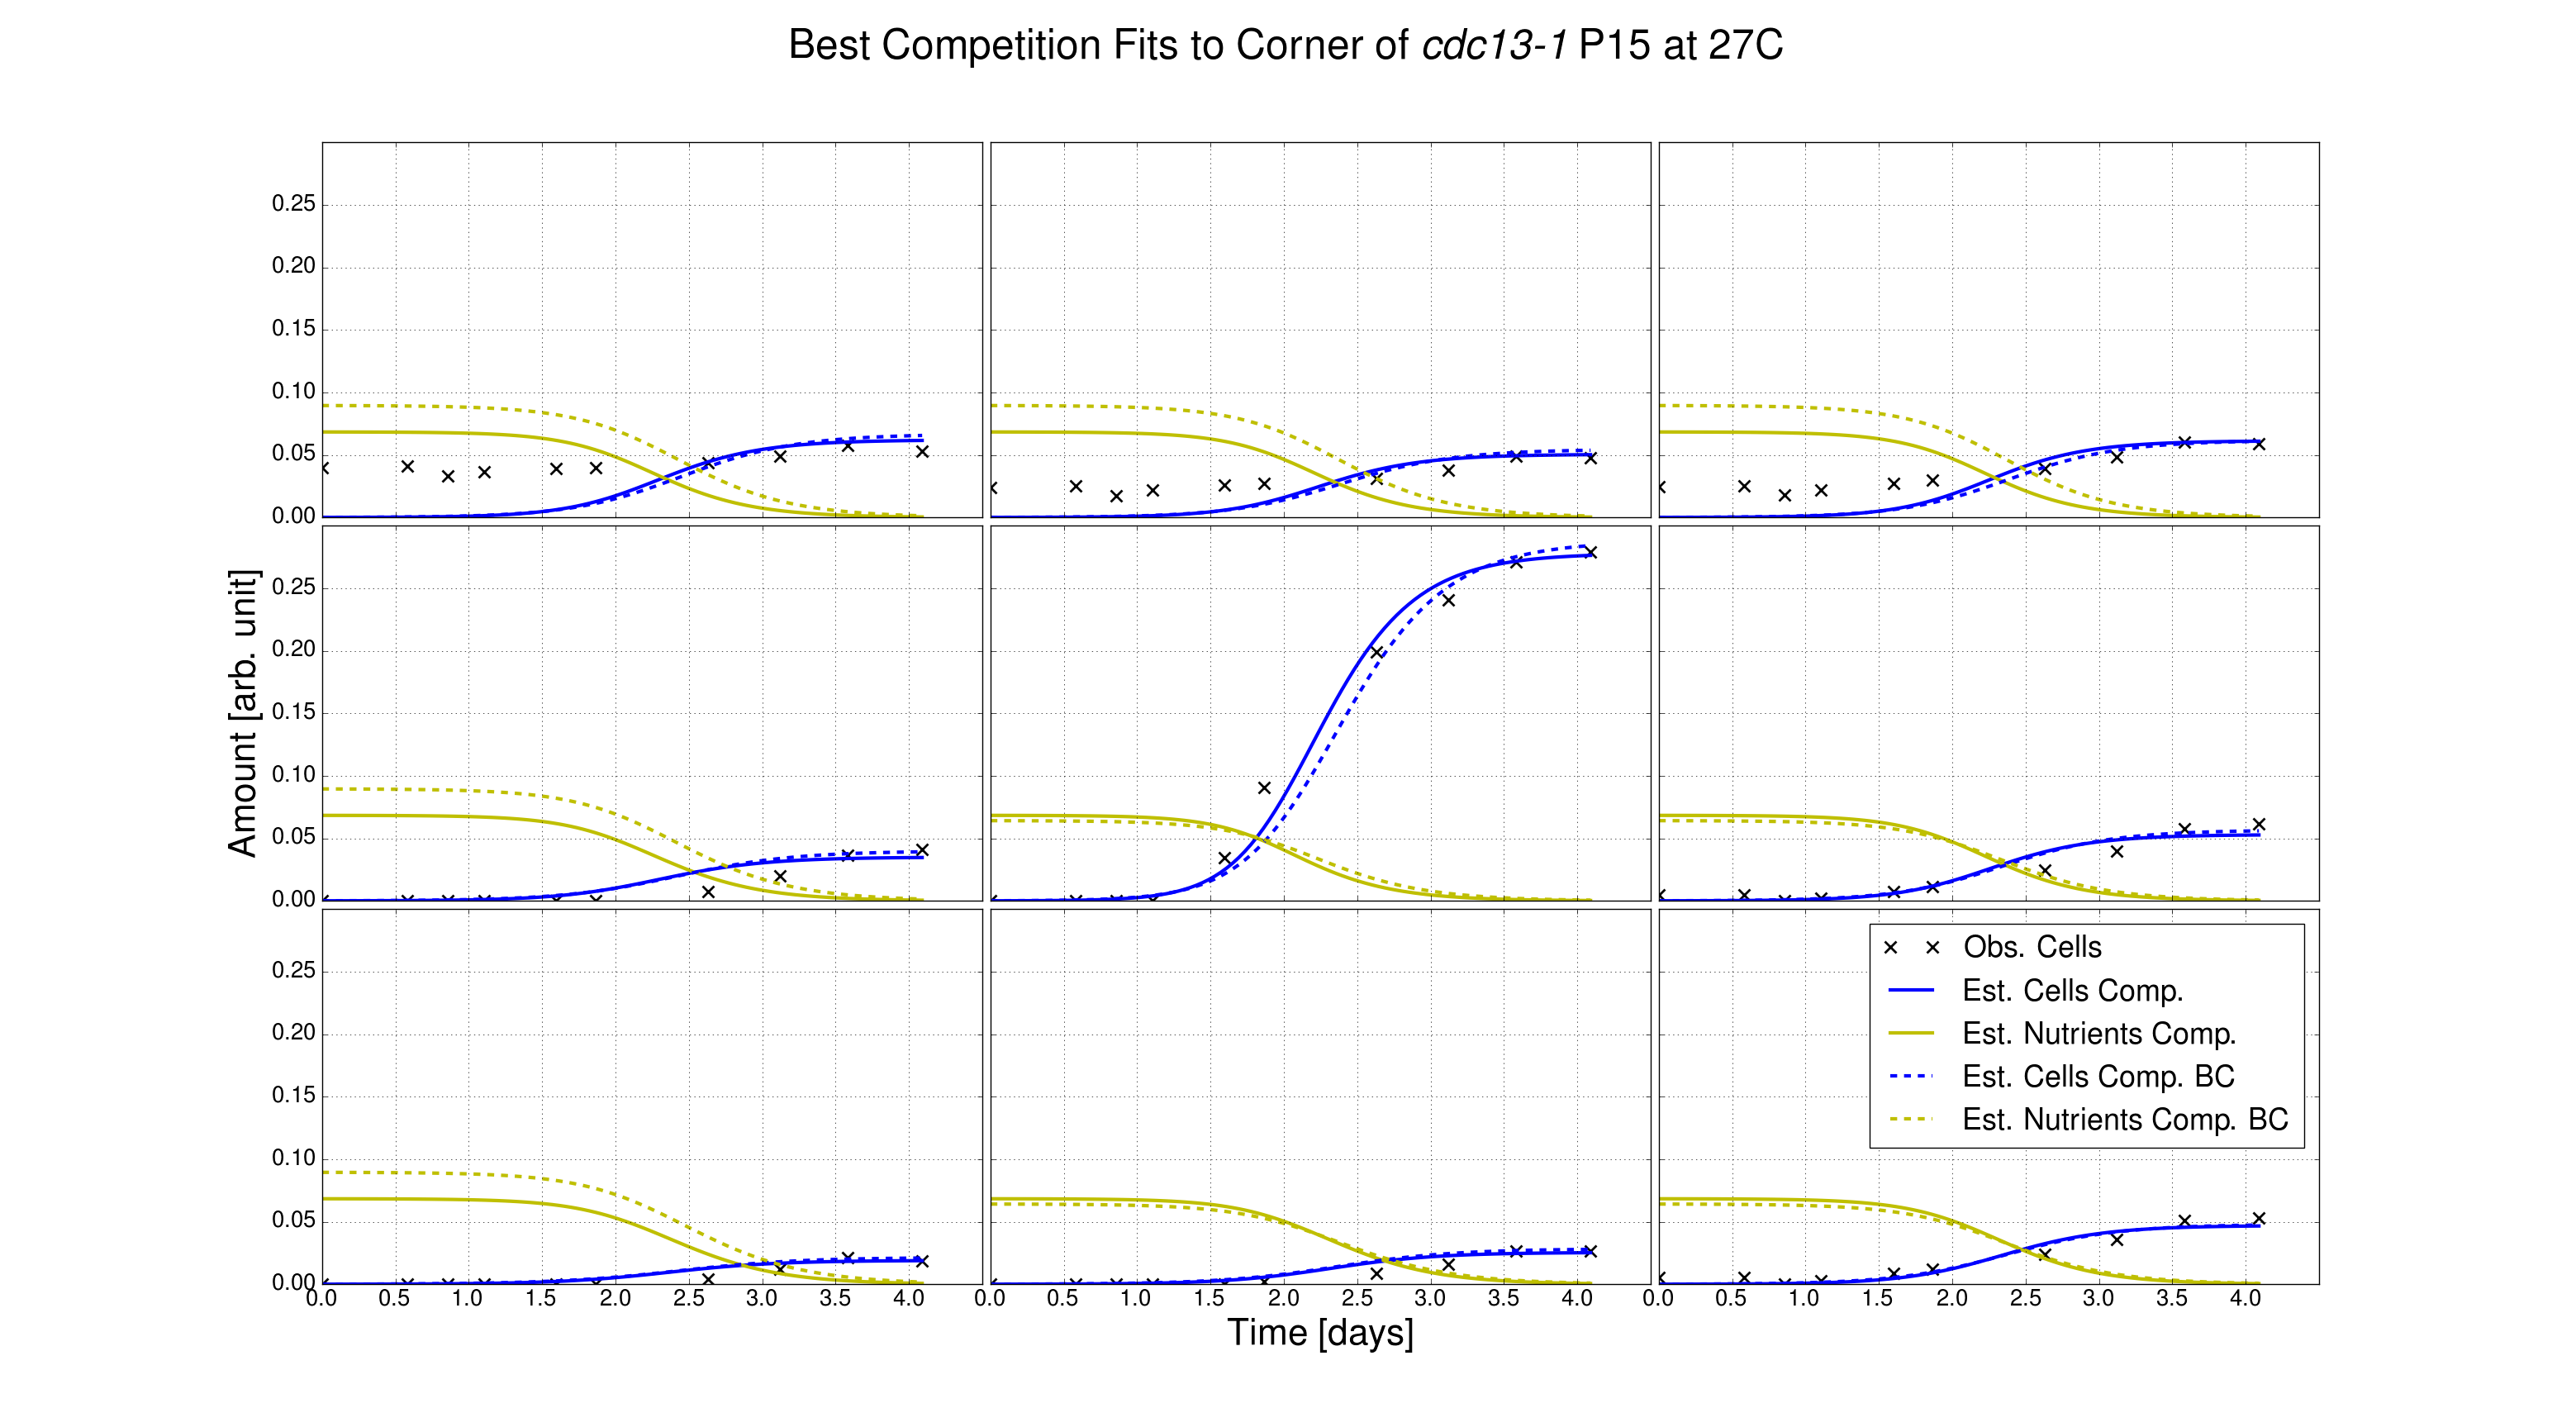
\includegraphics[width=\linewidth]{final/top_left}
  \captionof{figure}{\textbf{Treatment of boundary conditions in fits
      of the competition model.} The top left corner of a 16x24 QFA
    plate fitted with two versions of the competition model, the first
    has a single initial nutrient amount for all cultures, the second
    has a separate initial nutrient amount for edge cultures.}
  \label{fig:P15_corner}
\end{Figure}
\begin{multicols}{2}


\columnbreak
\begin{center}
  \captionof{table}{\textbf{Average error in objective function for
      one a two \(\bm{N_0}\) parameter competition models.} Values are
    for the same fits as in Figure~\ref{fig:P15_corner} and have been
    scaled by \(10^{4}\). Averages are for cultures belonging to the
    areas indicated by the column ``Cultures''. ``Next to edge''
    refers to cultures one in from the edge. ``Internal'' refers to
    all cultures but the edge.}
  \begin{tabular}{l l l}
    \hline
    Cultures     & One \(N_{0}\)  & Two \(N_{0}\) \\
    \hline
    Edge         & 35.9    & 36.5\\
    Next to edge & 9.54    & 7.98\\
    Internal     & 6.67    & 6.30\\
    All          & 12.4    & 12.2\\
    \hline
  \end{tabular}
  \label{tab:corner}
\end{center}
%\end{table}

Table~\ref{tab:corner}

  Some text Some text Some text Some text Some text Some text Some
  text Some text Some text Some text Some text Some text Some text
  Some text Some text Some text Some text Some text Some text Some
  text Some text Some text Some text Some text Some text Some text
  Some text Some text Some text Some text Some text Some text Some
  text Some text Some text Some text Some text Some text Some text
  Some text Some text Some text Some text Some text Some text Some
  text Some text Some text Some text Some text Some text Some text
  Some text Some text Some text Some text Some text Some text Some
  text Some text Some text Some text Some text Some text Some text
  Some text Some text Some text Some text Some text Some text Some
  text Some text Some text Some text Some text Some text Some text
  Some text Some text Some text Some text Some text Some text Some
  text Some text Some text Some text Some text Some text Some text
  Some text Some text Some text Some text Some text Some text Some
  text Some text Some text Some text Some text Some text Some text
  Some text Some text Some text Some text.

\subsection{\thesubsection~Agreement of b rankings}

\graphicspath{{images/rank/}}
\begin{Figure}
  \centering
  \includegraphics[width=\linewidth]{top_two_comp_p15_correlations_trimmed}
  \captionof{figure}{\textbf{Comparison of \(\bm{b}\) ranking for the
      best five competition model fits to P15.} Ranking is calculated
    from the mean \(b\) estimate from the six repeats or each strain.}
  \label{fig:comp_b_ranking}
\end{Figure}

\subsection{\thesubsection~Comparison of fitness ranking}

\graphicspath{{images/rank/}}
\begin{Figure}
  \centering
  \includegraphics[width=\linewidth]{final/comp_b_log_r_log_mdr_trimmed}
  \captionof{figure}{\textbf{Comparison of \(\bm{r}\) ranking for fits
      of the competition and logistic model to P15.} Competition model
    \(r\) was converted from \(b\), \(N_0\), and \(C_0\) from the best
    competition model estimate. Logistic \(r\) was taken from fits
    using the QFA R package which makes heuristic checks for slow
    growing cultures.}
  \label{fig:comp_vs_log_ranking}
\end{Figure}


\graphicspath{{images/rank/}}
\begin{Figure}
  \centering
  \includegraphics[width=\linewidth]{final/comp_b_log_r_trimmed}
  \captionof{figure}{\textbf{Comparison of \(\bm{r}\) ranking for fits
      of the competition and logistic model to P15.} Competition model
    \(r\) was converted from \(b\), \(N_0\), and \(C_0\) from the best
    competition model estimate. Logistic \(r\) was taken from fits
    using the QFA R package which makes heuristic checks for slow
    growing cultures.}
  \label{fig:comp_vs_log_ranking2}
\end{Figure}

\subsection{\thesubsection~Comparison of Variation in Fitness Estimates}

Use repeats on plate 15 (6 per deletion) to calculate coefficient of
variation (COV) of estimated r or MDR.

\end{multicols}
\graphicspath{{images/COV/}}
\begin{Figure}
  \centering
  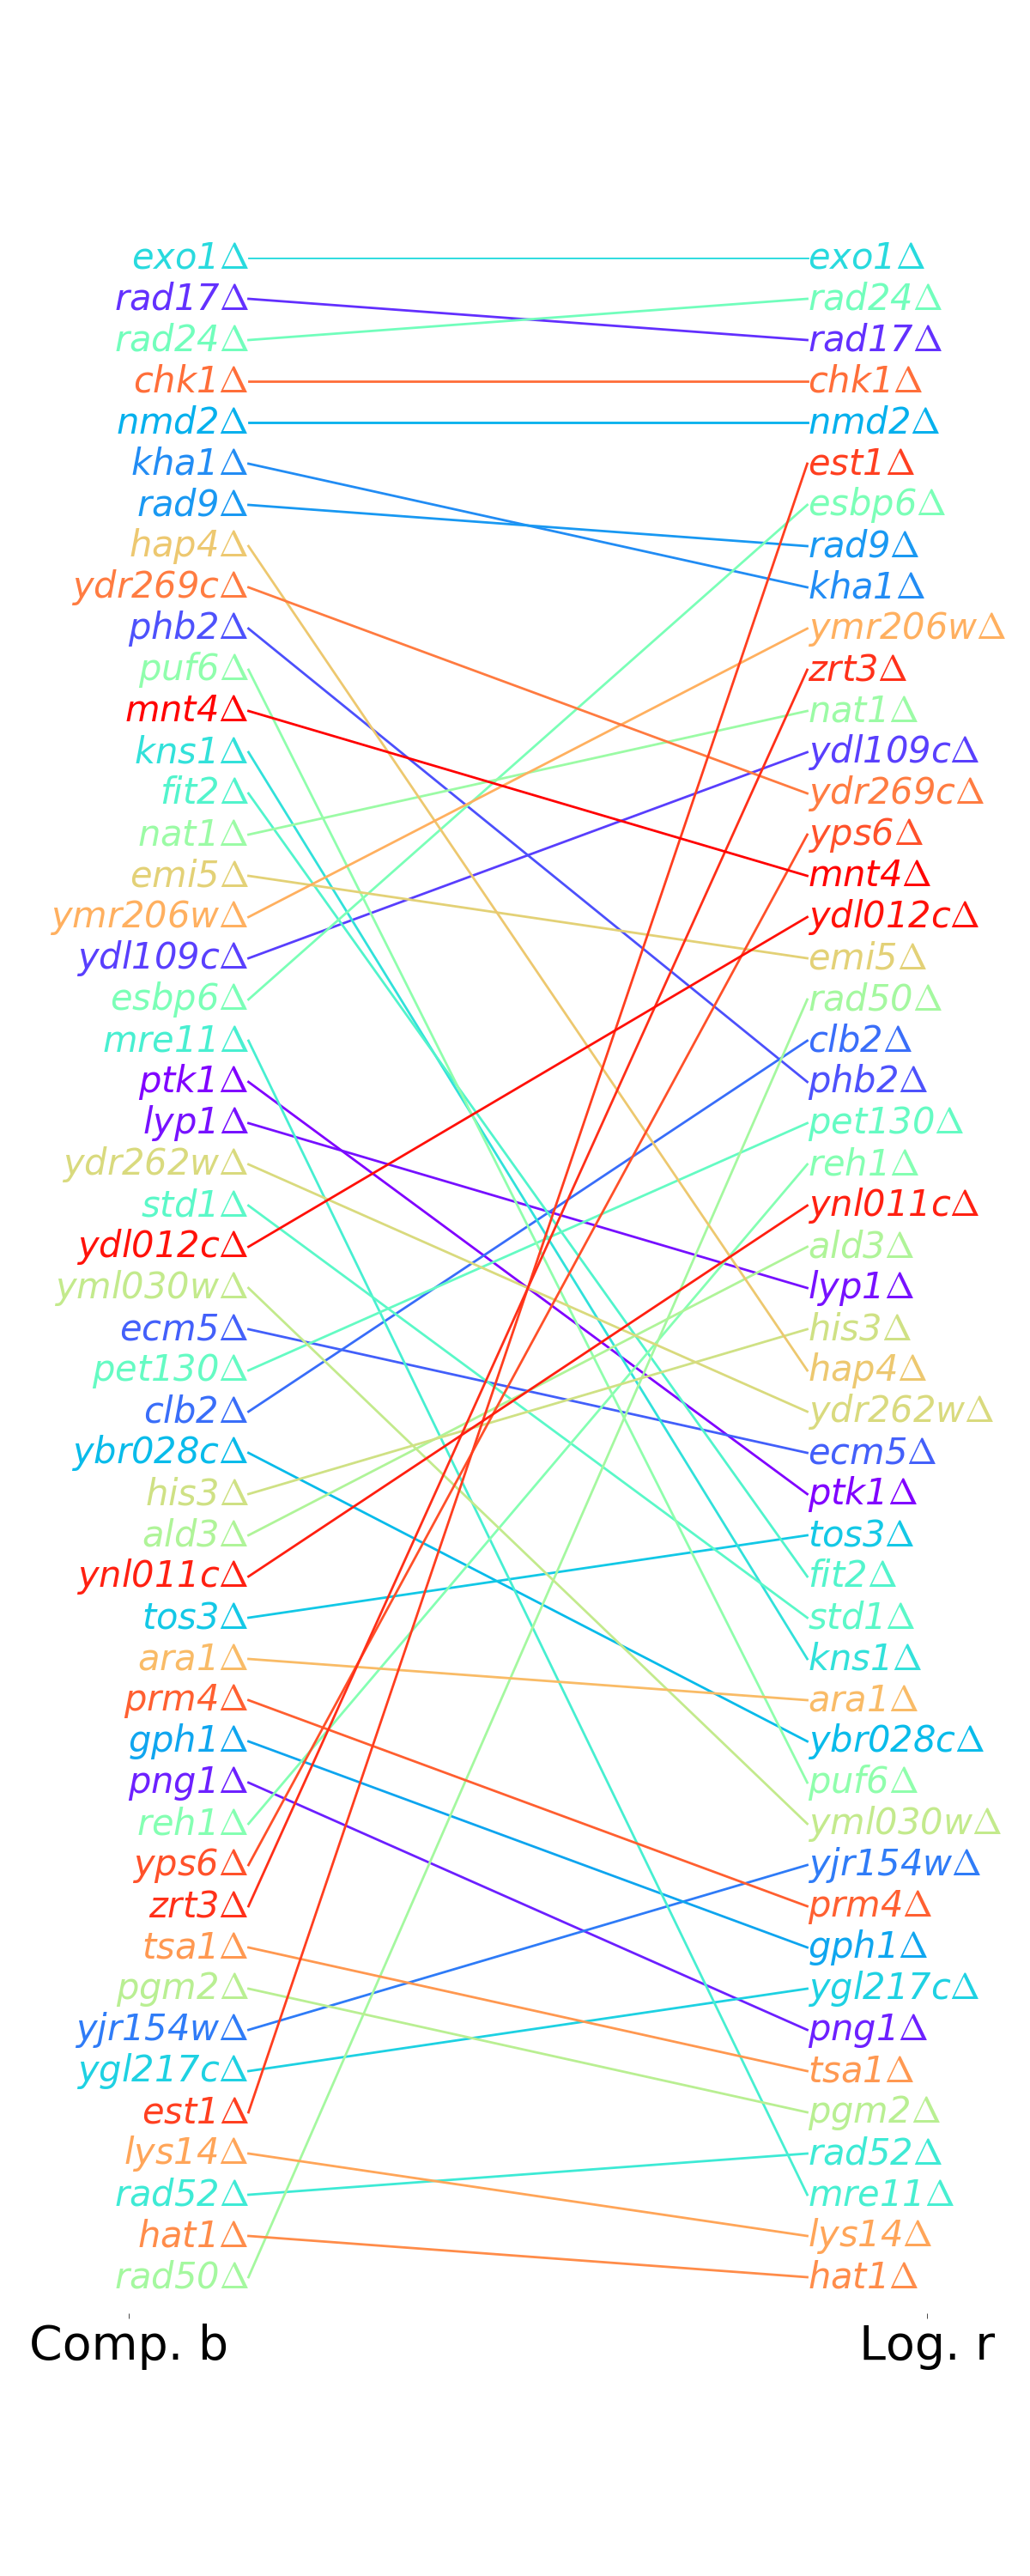
\includegraphics[width=\linewidth]{final/comp_b_log_r}
  \captionof{figure}{\textbf{Coefficient of variation of \(\bm{r}\)
      estimates.} Strains are ordered left to right along the
    horizontal axis by highest to lowest competition model \(r\)
    ranking. Fits are for the competition model, the QFA R logistic
    model, and the logistic equivalent model.}
  \label{fig:comp_b_log_r_cov}
\end{Figure}
\begin{multicols}{2}



\subsection{\thesubsection~Cross-plate validation}

\end{multicols}
\graphicspath{{images/stripes/}}
\begin{Figure}
  \centering
  \includegraphics[width=\linewidth]{final/validation_r9_c10_no_nutrients}
  \captionof{figure}{\textbf{Calibration and validation of the
      competition model.} I fit the competition model to the 16x24
    format ``Stripes'' and ``Filled'' plates in
    Figure~\ref{fig:stripes_images}. The plot shows cell measurements
    and estimates for both plates for a 3x3 section with top left
    coordinates (R9, C10). I took the parameters estimates for the
    ``Filled'' plate (calibration) and set growth constant, b, to zero
    for cultures in the empty columns of the ``Stripes'' plate. I then
    simulated using these parameters to produce the dashed blue curve
    (validation). If the model is working correctly, the dashed blue
    curve should resemble the ``Stripes'' data (blue crosses).}
  \label{fig:stripes_validation}
\end{Figure}
\begin{multicols}{2}


\graphicspath{{images/stripes/}}
\begin{Figure}
  \centering
  \includegraphics[width=\linewidth]{final/r_correlations_between_plates_A}
  \includegraphics[width=\linewidth]{final/r_correlations_between_models_B}
  \captionof{figure}{\textbf{Correlation of r estimates for
      ``Stripes'' and ``Filled'' plates.}~A) Correlation of r
    estimates between plates for logistic and competition
    models. B) Correlation of r estimates between logistic and
    competition models for both plates.  I fit the competition model
    and independent model to the ``Stripes'' and ``Filled'' plates in
    Figure~\ref{fig:stripes_images}. I converted competition model b
    to logistic model r. I only used data for cultures that were
    common between the two plates common and removed edge
    cultures. The Pearson correlation coefficient, \(\rho\), is shown
    in the legends. The line \(y=x\) is also plotted.}
  \label{fig:r_correlations}
\end{Figure}


\graphicspath{{images/stripes/}}
\begin{Figure}
  \centering
  \includegraphics[width=\linewidth]{final/r_correlations_between_plates_tight}
  \includegraphics[width=\linewidth]{final/r_correlations_between_models_tight}
  \captionof{figure}{\textbf{Correlation of r estimates for
      ``Stripes'' and ``Filled'' plates.}~I fit the competition model
    and independent model to the ``Stripes'' and ``Filled'' plates in
    Figure~\ref{fig:stripes_images}. I converted competition model b
    to logistic model r. I only used data for cultures that were
    common between the two plates common and removed edge
    cultures. The Pearson correlation coefficient, \(\rho\), is shown
    in the legends. The line \(y=x\) is also plotted.}
  \label{fig:r_correlations_v2}
\end{Figure}


\subsection{\thesubsection~Towards a genetic algorithm}

%\end{multicols}
\graphicspath{{images/genetic_algorithm/}}
\begin{Figure}
  \centering
  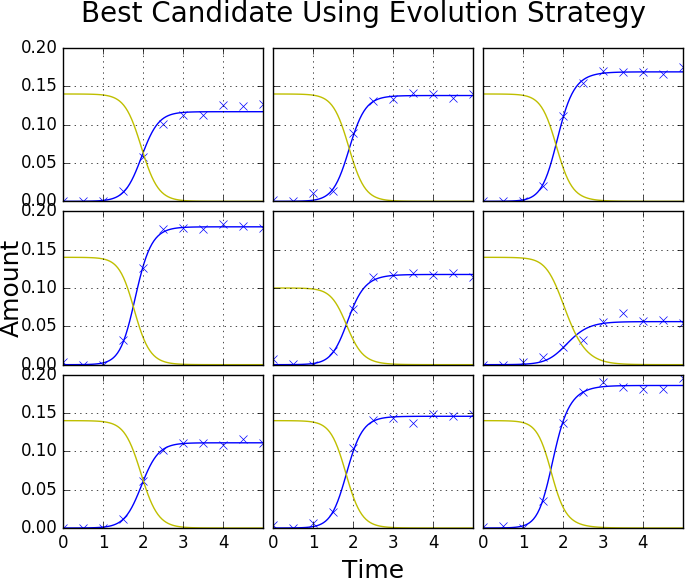
\includegraphics[width=\linewidth]{final/ga_fit_to_sim_true_plate_lvl_trimmed}
  \captionof{figure}{Genetic algorithm fit to a 3x3 simulation. MIGHT
    TAKE A LITTLE BIT OF WORK TO REPRODUCE AND COULD USE PARAMETERS
    FROM THE BEST P15 FIT RATHER THAN JUST PICKING/RANDOMIZING. NEED
    TO CHECK THAT PLATE LEVEL PARAMETERS WERE ALSO EVOLVED.}
  \label{fig:3x3_genetic_algorithm_comp_fit_fixed_plate_level}
\end{Figure}
%\begin{multicols}{2}


%\end{multicols}
\graphicspath{{images/genetic_algorithm/}}
\begin{Figure}
  \centering
  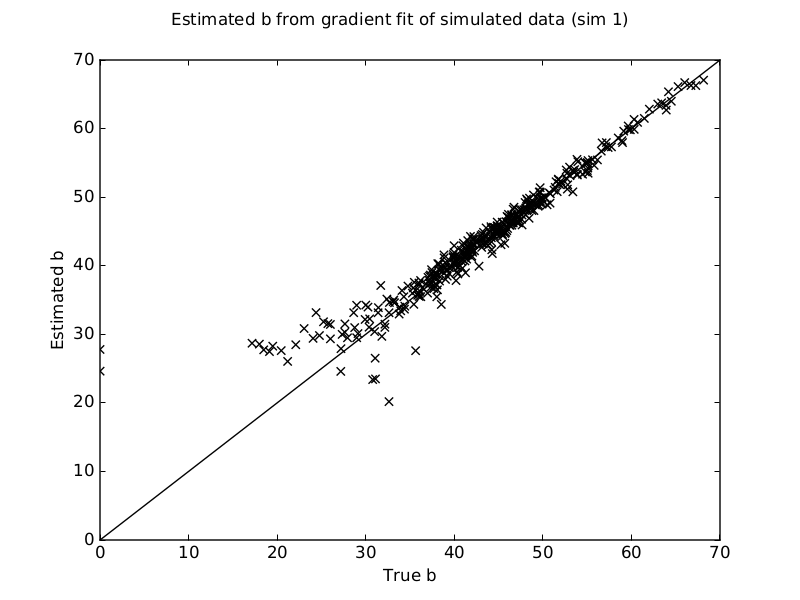
\includegraphics[width=\linewidth]{final/est_b_vs_true_b_imag_neigh_guess_sim_1_trimmed}
  \captionof{figure}{Recovery of true b values from a gradient method
    with fixed plate level parameters. I simulated timecourses from
    the best five (which model? all BC?) fits to p15, fixed the true
    plate level parameters, and used a gradient method to recover
    b. This plot shows the worst case from the five sets of values.}
  \label{fig:comp_fit_fixed_plate_level}
\end{Figure}
%\begin{multicols}{2}

%%% Local Variables:
%%% mode: latex
%%% TeX-master: "report"
%%% End:
